There are two primary methods of adjusting the problem size for determining its effects. The first method is to consider the full planning horizon, but to adjust the resolution (step size) used for planning. This method is referred to herein as ``slicing'' or ``sliced''. The second method is to only consider a shortened horizon at a fixed resolution or step size. This is referred to as the ``short'' method.

There are trade-off to the two methods, primarily concerning the resolution and horizon length for planning. A lower resolution (larger step size) can affect the quality of the solution (i.e., higher cost), due to the large times over which each control decision is applied and the potential for greater error introduced by the discretization method. A shorter horizon can lead to greater potential for planning difficulties or even infeasibility, as well as higher final costs (i.e., less optimal total solutions). A longer horizon time (short method) or higher resolution (sliced method), on the other hand, result in more optimization variables, which relates to the solve time of the optimization. The following sections investigate some of these relationships and trade-offs.

\subsection{Solve time} \label{ssec:solve_time}
As noted, the solve time of the optimization is related to the problem size in both the number of free variables, and the number of constraints. Due to the nature of this problem, both the number of variables and constraints grow with the increase in the number of discrete steps of the problem, for a given formulation of the problem. There is also a difference in the size of the problem between the methods of formulating the problem, with the QP formulation being the smallest, the LP-$\infty$ formulation the next smallest, and the LP-1 formulation the largest. The solve times for various numbers of discretization steps are compared for the various formulations (QP, LP-$\infty$, and LP-1) and methods (sliced and short).

As shown in Fig. \ref{fig:solve_time} the problem really starts to become burdensome to compute with a path of over 1000 steps. For both a QP (with Dual Simplex) and the LP formulations this is true, although more so for the QP. Note that solving the QP with the Barrier method is much faster (see Fig. \ref{fig:solve_time_barrier}), even at the largest problem size where the problem is solved in about 1 second compared to the ~15 and ~100 seconds for the LPs and QP w/Dual Simplex respectively. However, as the Barrier method cannot be used for the QP with mixed integers (i.e., obstacles) in Gurobi, it is more useful to understand the Dual Simplex solve time of the QP.

Also of note is the fact that the differences between the short and sliced methods are fairly negligible compared to the effect of both problem size and formulation. Additionally, the difference between the two LP formulations is fairly minimal comparative to the differences induced by the differing of the problem size. This indicates that the biggest factors affecting the solve time are the formulation type (i.e., QP vs LP) and the problem size.

\begin{figure}
    \centering
    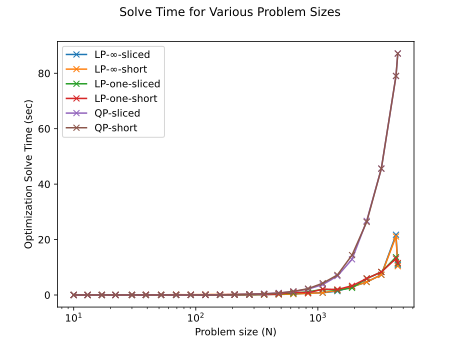
\includegraphics[width=\linewidth]{figs/solve_time.png}
    \caption{The solve time of the problem types and formulations over the problem size measured as the number of time steps in the horizon.}
    \label{fig:solve_time}
\end{figure}

\begin{figure}
    \centering
    \includegraphics[width=\linewidth]{figs/solve_time_barrier.png}
    \caption{The solve time where the barrier method is used for the QP rather than the dual-simplex method.}
    \label{fig:solve_time_barrier}
\end{figure}

\subsection{Objective Value} \label{ssec:obj_val}

There is a concern of the resolution (step size) of the sliced method affecting the quality of the solution. To investigate this, the resulting objective values at each resolution (corresponding to number of discretization steps) is compared. This requires some care, however, as the objective value is the sum of the weighted error at each discretization step. Changing the number of steps will naturally increase the objective value as there are more terms in the sum. Thus, to provide a fair comparison the objective value is multiplied by the step size in Fig. \ref{fig:norm_obj_val_dt}. The primary take away is that for nearly all step sizes the normalized objective value is nearly constant. Note that the cost differences between the different formulations are due to the different norms that correspond to the formulation, and are expected.

The ``weirdness'' of the end values is due to the fact that for a trajectory with an original number of 4516 steps and a step size of 0.01 seconds the only way to achieve a number of steps between $4516 \div 2 = 2258$ and 4516 by using the points from the original trajectory is to just use that many points from the trajectory along with the original step size. Thus, the trajectory for the last few points of the plot have the same step size but different number of steps in the trajectory. Thus, they have a different number of steps in the sum, but are being ``normalized'' with the same step size (0.01).

\begin{figure}
    \centering
    \includegraphics[width=\linewidth]{figs/costs.png}
    \caption{The step size versus the normalized objective value.}
    \label{fig:norm_obj_val_dt}
\end{figure}

The figure also shows that for low resolution (large step sizes) the value begins to be affected, and highly so in the cases of the LPs. It is unclear why the LPs are so highly affected when the QP formulation is not, and the effects for even lower resolutions were not investigated (the lowest resolution is at a step size of $\approx$4.5 seconds).


\subsection{Take-away} \label{ssec:prob_size_take_aways}

The most relevant results from investigating the effects of the problem size indicate that there is a range of problem sizes that constitute a sort of  ``sweet spot''. Using a resolution that is too low results in the solution quality being negatively affected, but using a larger problem size (potentially corresponding to a higher resolution) and the solve time begins to be too burdensome. While acceptable solve times vary by application, it is clear that much more that a problem size of $N=1000$ and the computational burden is likely to be too much, or very nearly so. A problem with a discretization step size greater than about one to two seconds, on the other hand, is likely to provide a solution that is of a low quality.

While the problem size and the resolution are not directly linked, they are implicitly connected and so the problem size and resolution limits provide upper and lower bounds of sorts. For example, in an MPC application where a fixed horizon length (in seconds, not number of steps) is desired, the resolution does directly correlate to problem size, and so there are upper and lower bounds on the resolution (problem size) based on the desired solve time, and the need for resulting solutions to be quality.
